
\chapter{Analysis}

In this section, we analyse \zclaim from different perspectives.
In \cref{sec:sec_analysis}, we show that the protocol fulfills certain properties under which we consider it to be secure.

In \cref{sec:attack_vs}, we present several common attack vectors on blockchain protocols and discuss their (in-)feasibility on \zclaim, providing thresh\-old parameters guaranteeing the security of the system where appropriate.

Finally, in \cref{sec:privacy}, we analyse privacy concerns related to the vault intermediary system.


\section{Security analysis}
\label{sec:sec_analysis}

In this section, we present a set of properties under which \zclaim is considered secure.
We specify the conditions that need to hold in order to attain each of these properties.
Finally, we show that \zclaim satisfies these conditions.

We presuppose the proper choice of security parameters $k^I$, $k^B$, $\Delta^I$ and $\Delta^B$ as discussed in \cref{sec:setup} and the security of the Zcash/Zerocash protocol, which has been extensively shown in~\cite{sasson2014zerocash}.
We also assume that the relay system is secure and that if a block header is accepted by the relay system, the possibility of a future chain reorganisation is vanishingly low.

\subsection{Notation}

We denote any participant in the protocol by $P \in \mathcal{P}$, who may be a vault $V \in \mathcal{V}$ or a user $U \in \mathcal{U}$ taking on the role of issuer or redeemer.
The amount of currency X of any of the backing currency Zcash (ZEC), the issuing chain's native currency (\emph{ICN}) and the issued currency (\emph{ICZ}) that a participant can spend is denoted by $X(P)$, e.g.\ $ICN(U)$, to which we may refer to as $U$'s ICN \emph{balance}.
Specifically, $ZEC(P)$ is the sum of the value of all unspent Zcash notes of which $P$ has knowledge containing $\dpa_P$, the diversified payment address associated with $P$.
Same goes for ICZ.
Funds locked as collateral by participant $P$ are denoted by $X^{col}(P)$.

In addition to the aforementioned balances, $ZEC^{obl}(V)$ are the \emph{ZEC obligations} associated with vault $V$ and is defined as the sum of the ZEC value of all (hidden) amounts of ICZ issued or redeemed in \mint and \burn transactions facilitated by $V$.
This also represents the amount that vaults can release to redeemers and does not reflect their ZEC balance, since $ZEC(V)$ includes the fees accumulated by $V$ in past transactions while $ZEC^{obl}(V)$ does not.
Furthermore, it is not possible to verify that $ZEC(V)$ matches $ZEC^{obl}(V)$ in any way as $V$ may perform arbitrary shielded transactions at any time.

Upon submission of a valid POB (or similarly for POCs), in which a vault proves in zero knowledge that $c \geq ZEC^{obl}(V) \cdot \xr \cdot \sstd$ where $c \leq ICN^{col}(V)$, $V$ is said to have some \emph{blocked collateral} $ICN^{bcol}(V) = ZEC^{obl}(V) \cdot \xr \cdot \sstd$ and some free collateral $ICN^{fcol}(V) = c - ICN^{bcol}(V)$.
The vault's blocked collateral are the funds backing their ZEC obligations, which they can only decrease by releasing funds to users (or by burning ICZ, see discussion on rebalancing in \cref{sec:rebalancing_exit}).

$X_t(P)$ denotes P's balance at time $t$, where one step in time corresponds to a transaction on I.
$ZEC_t(P)$ is not defined.

Finally, $\xr_t$ denotes the latest ZEC to ICN exchange rate as provided by the exchange rate oracle \oxr at time $t$, where 1 ZEC = $\xr_t$ ICN.
We assume a 1:1 peg between the issued currency and the backing currency, i.e.\ 1 ZEC = 1 ICZ.

\subsection{Goals}
\label{sec:security_goals}

We deem \zclaim \emph{secure} if it achieves the following properties:
\begin{itemize}
    \item \textbf{Soundness} The amount of issued currency in circulation is equal to the amount of ZEC obligations, i.e.\ for all $t \geq 0$
    \begin{equation}\label{eq:icz_equals_obl}
        \sum_{U \in \mathcal{U}} ICZ_t(U) = \sum_{V \in \mathcal{V}} ZEC^{obl}_t(V)
    \end{equation}
    and $ZEC^{obl}(V)$ is derived from protocol transactions to and from $V$ on Zcash.
    Specifically,
    \begin{lemma}\label{le:lock_before_mint}
        For every Mint transfer of (hidden) value $\val_{IM}$ on I containing $\dpa_V$ as the vault's diversified payment address, there is an Output transfer on Zcash creating a note of value $\val_Z$ to $\dpa_V$ s.t.
        \begin{equation}
            \left \lfloor{\val_Z \cdot (1 - f)}\right \rfloor = \val_{IM}
        \end{equation}
    \end{lemma}
    and
    \begin{lemma}\label{le:release_before_burn}
        For every Burn transfer of value $\val_{IB}$ on I containing $\dpa_V$ as the vault's diversified payment address and $\cm_Z$ as the requested release note commitment, there is an Output transfer on Zcash creating a note of value $\val_Z$ with note commitment $\cm_Z$ s.t.
        \begin{equation}
            \val_Z = \left \lfloor{\val_{IB} \cdot (1 - f)}\right \rfloor
        \end{equation}
    \end{lemma}
    according to the fee policy defined in \cref{sec:fees}.
    
    These are the transfers that make up a vault's ZEC obligations, and evidently the sum of all Mint transfers minus all Burn transfers is equal to the circulating supply.
    Hence \cref{eq:icz_equals_obl} is in fact satisfied by the definition of $ZEC^{obl}(V)$.
   
    \item \textbf{Coverage} The total amount of ZEC obligations are backed by a proportional amount of the issuing chain's native currency according to the prevailing exchange rate, i.e.\ for all $t \geq 0$
    \begin{equation}\label{eq:coverage}
        \left(\sum_{V \in \mathcal{V}} ZEC^{obl}_t(V)\right) \cdot \xr_t \cdot \smin \leq \sum_{V \in \mathcal{V}} ICN^{bcol}_t(V)
    \end{equation}
    where $\smin$ is the minimum collateralisation ratio as defined in \cref{sec:constants}.
    
    \item \textbf{Fairness} An honest participant following best practices will not incur any loss of funds as long as they can receive and broadcast transactions from and to chains Z and I.
    
    For the condition on this claim, availability of both chains must be guaranteed, which we derive from the security assumption of \xclaim that transactions broadcast by users are received by (honest) consensus participants within a known maximum delay $\Delta_{tx}$.
    In case of network failure for a significant amount of time on the user/vault side, they may in effect incur loss of funds.
    It is thus the participants' responsibility to ensure they remain online throughout the duration of a subprotocol.

    As for the claim itself, we examine the cases where a participant may incur loss of funds.
    This risk exists both in the issue and redeem subprotocols.
    We concern ourselves with transactions that incur a change in any of the balances of the two parties involved (except for slashing, which we cover separately) i.e.\ in which a monetary transaction takes place.
    These are, on the one hand, \lock and \release transactions, and on the other, \mint and \burn transactions.
    
    Concerning the issue subprotocol, the following statements must be proven:
    \begin{lemma}\label{le:mint_after_lock}
        After executing a lock operation, a user is able to mint the locked amount minus fees of ICZ.
    \end{lemma}
    \begin{lemma}\label{le:lock_before_mint2}
        If a \mint transaction involving a vault $V$ is confirmed on I (thus increasing their ZEC obligations), $V$ has received the amount being minted plus fees in a previous \lock transaction.
    \end{lemma}
    Note that \cref{le:lock_before_mint2} is equivalent to \cref{le:lock_before_mint} with the added requirement that $V$ must have knowledge of the note values.
    
    Analogously, for redeeming we must show that:
    \begin{lemma}\label{le:burn_after_release}
        After executing a release operation, a vault is able to trigger the inclusion of an associated pending \burn transaction decreasing their ZEC obligations by the released amount plus fees.
    \end{lemma}
    \begin{lemma}\label{le:release_before_burn2}
        If a \burn transaction involving a user $U$ is confirmed on I, $U$ has received the amount being burned minus fees in ZEC in a previous \release transaction.
    \end{lemma}
    Again, \cref{le:release_before_burn2} is tantamount to \cref{le:release_before_burn} with addition of the knowledge requirement.
    
    Consideration must additionally be paid to the slashing mechanism, in order to ensure that slashing of an honest party cannot be instigated by a malicious one.

    Finally, we provide a set of practices that vaults may follow in order to prevent liquidation and hence loss of funds.
\end{itemize}

\subsection{Argumentation}

We show that \cref{le:lock_before_mint,le:release_before_burn} are always satisfied and, furthermore, that the recipients of the Zcash notes referenced therein have knowledge of the note values, hence satisfying \cref{le:lock_before_mint2,le:release_before_burn2}.
Further, we cover \cref{le:mint_after_lock,le:burn_after_release}, and show the validity of \cref{eq:coverage}.
Finally we discuss slashing and liquidation.

\subsubsection{Issuing}

The zk-SNARK $\pim$ in Mint transfers as defined in \cref{sec:mint} guarantees that \cref{le:lock_before_mint} holds through the \textbf{Note commitment integrity} condition together with the Merkle path validity success requirement (there exists such a note on Zcash), and the \textbf{Locked value}, \textbf{Minted value} and \textbf{Fee rounding commitment integrity} conditions (the note has the specified value).

Mint transfers also satisfy \cref{le:mint_after_lock} through \textbf{Trapdoor commitment integrity}, which guarantees that only the user that authored the \lock transaction can create a \mint transaction.

Furthermore, the challenge mechanism guarantees that the vault has knowledge of the note values, satisfying \cref{le:lock_before_mint2}, since \mint transactions will only be included on I if they are not successfully challenged.
The vault can challenge the pending transaction through disclosure of the shared secret, proven to be correct in $\pic$.
If the note values have not been correctly encrypted to the vault, the transaction will be discarded, which ensures \textbf{Fairness}.

So far we have proven \cref{le:lock_before_mint,le:mint_after_lock,le:lock_before_mint2}.

\subsubsection{Redeeming}

Equally, the conjunction of $\pib$ as defined in \cref{sec:burn} and the \confirmRedeem transaction guarantees that \cref{le:release_before_burn} holds through the conditions in \pib and the Merkle path validity success requirement of \confirmRedeem transactions.

\Cref{le:burn_after_release} is rather trivial as all it takes is to provide a Merkle path showing the existence of the note commitment in the note commitment tree, which not only the vault but any participant can do.

As for redeeming, the challenge mechanism works somewhat differently: it is the recipient of the note (the redeemer) who constructs it, and the sender must have knowledge of the values in order to be able to create it.
Thus \cref{le:release_before_burn2} is satisfied by construction, and we can move on to the challenge mechanism: in this case, it serves to ensure the vault has received the correct note values.

A vault may successfully challenge the transaction if and only if the provided note commitment cannot be generated from the decrypted values, thus it cannot punish honest redeemers but also a redeemer cannot ask a vault to release a note it cannot create, causing it to be slashed.
Hence \textbf{Fairness} is ensured when redeeming too.

Now, we have also proven \cref{le:release_before_burn,le:burn_after_release,le:release_before_burn2}, in addition to \cref{le:lock_before_mint,le:mint_after_lock,le:lock_before_mint2} from before, which concludes the proof for \textbf{Soundness}.
It remains to prove \textbf{Coverage} and to discuss loss of funds in liquidations and challenge operations.

\subsubsection{Proofs of balance}

From \cref{eq:coverage} it is evident that if we can show that 
\[
    ZEC^{obl}_t(V) \cdot \xr_t \cdot \smin \leq ICN^{bcol}_t(V)
\]
for any vault, then~\eqref{eq:coverage} holds for the entire system.

We recall here that $ICN^{bcol}(V) = ZEC^{obl}(V) \cdot \xr \cdot \sstd$, which nevertheless only holds for some $\xr$ used in the POB.
We shall denote this exchange rate by $\xr_V$.

Technically, it also only holds for $ZEC^{obl}(V)$ at the time of its last POB, though the only problematic case is that in which a vault's ZEC obligations increase since that time, i.e.\ they issue funds.

However, vaults may only become available to issue by submitting a POC (and must provide POCs instead of POBs until issuing is completed), in which they prove collateralisation for their ZEC obligations plus the maximum amount they can issue in one round.
Thus we may assume without loss of generality that $ZEC^{obl}(V)$ stays constant.

For any $\xr_t > \xr_V$ then it must hold that
\[
    ZEC^{obl}(V) \cdot \xr_t \cdot \smin \leq ZEC^{obl}(V) \cdot \xr_V \cdot \sstd
\]
\[
    \xr_t \cdot \smin \leq \xr_V \cdot \sstd
\]
which is the liquidation trigger as defined in \cref{sec:liquidation}.

Liquidation reduces $V$'s ZEC obligations until they meet \sstd again as described in the aforementioned section.

Thus we see that~\eqref{eq:coverage} does indeed always hold and is enforced by reducing the circulating supply if needed through liquidation auctions.
This concludes the proof for the \textbf{Coverage} property.

\subsubsection{Challenging}

Challenge operations result in the challenged party's warranty collateral $ICN_w$ being transferred to the challenging party if successful (for vaults, this amount is deducted from their staked collateral).
However, by definition these are only successful if the note plaintext in the challenged transaction has not been correctly encrypted to the challenger.
Thus it is not possible to cause loss of funds through these operations to an honest participant that adheres to the protocol.

\subsubsection{Liquidation}
\label{sec:analysis_liquidation}

In the event of liquidation, vaults are effectively slashed the liquidation penalty on the funds sold through the liquidation auction.
The amount of funds sold depends on the collateralisation constants and is always a fixed fraction of the vault's total collateral.

As mentioned in \cref{sec:liquidation}, with the collateralisation constants as suggested, liquidation is triggered on a vault if the exchange rate increases by 33\% with respect to $\xr_{V}$, the last exchange rate they used in a proof of balance.

In order to avoid liquidation, $V$ needs to provide a POB using a higher $\xr$ before the aforementioned threshold is reached.
If at any time $t$ where $T_{p} < t < T_{liq}$ and $\xr_{V} < \xr_t < \xr_{T_{liq}}$, it holds that
\begin{equation}\label{eq:pob_requirement}
    ZEC^{obl}_t(V) \cdot \xr_t \cdot \sstd \leq ICN^{col}_t(V)
\end{equation}
the vault can submit a new POB using $\xr_t$, hence avoiding liquidation at $T_{liq}$.
Naturally, this holds for later steps in time: if the exchange rate further increases, the vault will need to continue providing POBs in order to protect themselves from liquidation.
Vaults should choose a sensible $\xr_t > \xr_{V}$ for which to submit a new POB before they approach the liquidation threshold.

However, if \cref{eq:pob_requirement} is no longer satisfied, i.e.\ the change in the exchange rate at time $t$ has caused $V$'s collateralisation rate to fall below $\sstd$, $V$ first needs to top up their collateral or rebalance in order to be able to submit a POB using $\xr_t$.

If they hold ICN such that $ZEC^{obl}_t(V) \cdot \xr_t \cdot \sstd \leq ICN^{col}_t(V) + ICN_t(V)$, this is straightforward (barring the case where the exchange rate further increases such that \cref{eq:pob_requirement} again does not hold after collateral has been topped up) and is accomplished in the time it takes the vault to construct the two transactions and forward them to the network, which is negligible.

However, if this is not the case, $V$ may first have to acquire some $ICN$ to top up their collateral such that they can again submit a POB.
How long it takes them to do so depends on many external factors, but it may plausibly be up to several days: they may first have to procure liquid assets, transfer them to an exchange, trade them for ICN, withdraw the ICN from the exchange and finally lock them as collateral.
In this case, it may be fair to say that all is lost and vaults should follow best practices in order to avoid this sort of situation.

Another option vaults have to satisfy \cref{eq:pob_requirement} is to rebalance, but this is a strictly longer process than topping up their collateral since it also requires ICN and one further transaction on $I$, but also exchanging ICN for ICZ.
Thus if the goal is for them to protect themselves from liquidation as fast as possible, they should always choose to top up.
In addition to this, vaults may choose to start rebalancing such that they do not need to top up again if the exchange rate further increases or that they may unlock some collateral again.

Best practices vaults can follow in order to protect themselves from liquidation may thus include:
\begin{itemize}
    \item Maintaining a collateralisation rate somewhat higher than $\sstd$, i.e.\ overcollateralising, by strategically advertising themselves only to issue or redeem, rebalancing or increasing their collateral when necessary.
    For example, $\sigma_{sft} = 2$.
    \item Holding some amount of ICN not locked as collateral that they may use to top up their collateral or rebalance, or ensuring that they may acquire such amount quickly in case of emergency.
    \item Submitting POBs to address changes in the exchange rate above a certain threshold $r_{\xr} = \frac{\xr_t}{\xr_V}$.
    This should be a value close to $1.0$, e.g.\ $r_{\xr} \leq 1.05$.
\end{itemize}

Vaults may modify these parameters according to their risk tolerance, but with the suggested values we observe that for liquidation to be triggered it would be necessary that $\frac{\xr_t}{\xr_V} > \frac{\sigma_{sft}}{\smin} - r_{\xr} \approx 1.62$ i.e.\ the exchange rate increases by 62\% before $V$ is able to acquire new funds or rebalance.

Such a dramatic increase is unlikely to happen in a short time window, but in the context of cryptocurrencies, where high volatility is the norm rather than the exception~\cite{Lahmiri2018LongrangeMDvolatility,CAPORALE2019143volatility}, it is impossible to set a definite threshold for the increase in the exchange rate above which the likelihood of it taking place is insignificant.
Ultimately, it is left to vaults to assess the risks themselves.

Finally, liquidation may also be triggered if a vault fails to comply with issue or redeem requests too often, which should however not happen under the availability assumptions of participants under which \textbf{Fairness} applies.

Thus if we make the assumption that \xr will not increase fast enough to trigger liquidation on vaults following best practices, this concludes the argumentation in favour of \textbf{Fairness}.

\section{Attack vectors and points of failure}
\label{sec:attack_vs}

We discuss here a range of attacks and points of failure in \zclaim and offer mitigation strategies.
Familiarity with the security analysis of \xclaim~\cite[Section~VII]{zamyatin2019xclaim} is assumed.
Where not specified otherwise, the discussion on specific vulnerabilities offered there also holds for \zclaim.

\subsection{Inference attacks}
\label{sec:inference_attacks}

As discussed in \cref{sec:privacy}, vaults may guess the users' identity through the amounts in \lock and \release transactions in which they are involved.
The knowledge of this amount is of course per se insufficient to this end, but it can lay the ground for an inference attack leading to de-anonymisation if combined with other information they may have access to.

For instance, if an easily identifiable amount a user locks with a vault matches a recent transparent-to-shielded transaction on Zcash, the vault may deduce that there is a high likelihood those two transactions were performed by the same user.
This is similar to the heuristic used by \textcite{quesnelle2017linkability} to identify what he calls \textcquote[1]{quesnelle2017linkability}{round-trip transactions, where the same, or nearly the same number of coins are sent from a transparent address, to a shielded address, and back again to a transparent address. [He argues that] such behavior exhibits high linkability, especially when they occur nearby temporally}.
If the vault is correct in their assumption, they may be able to infer the user's identity from previous and future activity associated with the disclosed transparent address.

Another possibility is the case where a vault has privileged access to other information on one or many users, such as through data from a cryptocurrency exchange.
This may render them capable of effortlessly matching the real-world identities of exchange users with specific \lock or \release transactions if, for example, the guessed/observed amount matches a recent withdrawal from the exchange.

In both of these scenarios, an attacker may leverage this information to attempt extortion or defamation of the involved parties.

The splitting strategy defined in \cref{sec:splitting_strategy} aims to prevent this sort of attacks.
\zclaim's privacy has been analysed in this context in \cref{sec:privacy}.

\subsection{Chain relay poisoning}
\label{sec:relay_poisoning}

Chain relay poisoning involves an adversary triggering a chain reorganisation, or \emph{reorg} for short, of $N \geq k^B$ such that a previously accepted transaction at depth $N$ is invalidated.
This is known as an $N$-confirmation double spend and yields similarities to selfish mining~\cite{eyal2014majority} in that it involves misleading honest nodes through an amassing of computational power.

We recall here that the security parameter $k^B$ is based on the assumption that an adversary's computational power is bounded by $\alpha \leq 33\%$ and denotes the depth at which the likelihood of an adversary triggering a reorg is negligible.

However, in \xclaim a poisoning attack may be successful well below this threshold $\alpha$ if the relay system is deprived of recent block header data~\cite[Section VII-A]{zamyatin2019xclaim}.

We expand here on this observation.
This is in fact a common vulnerability to cross-chain interoperability schemes and is not only the case if the relay system is devoid of real-world data~\cite{2017hijackingbtc}, but may involve more intricate attacks in which \emph{relayers} are isolated from the rest of their peers in the network and misled to accept the attacker's chain as the longest.
This is more commonly known as an eclipse attack~\cite{heilman2015eclipse}.

Such attacks along with mitigation strategies have been discussed previously in the literature~\cite{heilman2015eclipse,wust2016ethereum,xu2020eclipsed,alangot2020decentralized}, and we refer the reader in particular to analyses on Bitcoin and Bitcoin-based blockchains (such as Zcash is) for mitigation strategies~\cite{heilman2015eclipse,alangot2020decentralized}.

\subsection{Exchange rate poisoning}
\label{sec:er_poisoning}

Similarly, if \oxr is manipulated to provide an erroneous price feed, this may allow a prepared adversary to steal funds in several ways.

For instance, an exchange rate much higher than the actual value would allow vaults to issue ZEC or unlock collateral such that they become undercollateralised when the exchange rate returns to normal.
An economically rational vault would have no incentive to bring back their collateralisation rate above the safety value and may choose to undergo liquidation and retain the ZEC for which they hold obligations, effectively violating \textbf{Soundness} and jeopardising the stability of the protocol.

On the other hand, an artificially low exchange rate may trigger mass liquidation and allow users to buy vaults' collateral at an unfair price, hence stealing funds from them.

It is thus of paramount importance to guarantee the reliability of the exchange rate oracle.
Blockchain oracles aim to solve this exact problem~\cite{peterson2015augur,8726819astraea,ellis2017chainlink}, aggregating exchange rates from different sources, leveraging economic incentives to reinforce the veracity of these sources and providing dispute mechanisms in case of discrepancies.
These systems are, without question, safer than relying on a single source to provide an exchange rate, though they may still fail under certain circumstances~\cite{lo2020reliabilityoracles}.

Further measures can be taken to prevent such an attack, such as sanitising data provided by the oracle or employing so-called circuit breakers~\cite{2019circuitbreakers}, which involve halting operations in case of unusual price movements.

Lastly, it must be noted that relying on a decentralised oracle constitutes a further cross-chain integration and as such opens another door to poisoning attacks as discussed in the previous section, which can be addressed through the same countermeasures.

\subsection{Replay attacks on inclusion proofs}

\zclaim prevents replay attacks on \lock and \release transaction inclusion proofs, in which a user reuses a past \lock transaction to mint ICZ or a vault reuses a \release transaction to decrease their ZEC obligations, stealing funds from the other party, as follows.

The nonce $\nlock$ provided by the issuing chain in lock permits must be used to generate the note commitment trapdoor in \lock transactions as specified in \cref{sec:lock}, which is enforced in the zero knowledge proof in Mint transfers $\pim$ through the \textbf{Trapdoor commitment integrity} condition.
This ensures that every \lock transaction is uniquely associated with the corresponding Issue procedure.

As for \release transactions, protection from replay attacks is implicit since the note commitment is generated in advance by the redeemer.
Therefore a vault can only replay a release inclusion proof if the redeemer has chosen the same note values, most notably the same note commitment trapdoor \rcm as in a previous Burn transfer.

However, the likelihood of the same trapdoor being sampled twice randomly from $\ncm.\gent$ as specified in \cref{sec:release} is insignificant.
If a redeemer purposely reuses the same note values, they only derive negative utility from their actions.

\subsection{Counterfeiting}
\label{sec:counterfeiting}

In \xclaim, counterfeiting is defined as the issuing of issued currency that is not backed by funds locked with vaults.
This is enforced through the principle of \textbf{Auditability}.
In a nutshell, since the vaults' actions are observable by anyone, a vault removing funds from the pool of funds locked with them can be reported and will be punished by slashing their collateral as a consequence.
This also includes vaults reusing these funds to mint more issued currency.

It is here that a central difference between \zclaim and \xclaim arises: we do not make such restriction.
Instead, \textbf{Coverage} and \textbf{Soundness} guarantee that the total amount of issued currency in circulation is always backed by an equivalent amount of the vaults' collateral.
A vault may very well reuse ZEC locked with them to issue more ICZ; they will still be unable to unlock their collateral until they have released ZEC to redeemers or burnt ICZ themselves.

Counterfeiting would hence imply issuing ICZ which is not locked by ICN, which is impossible as per the aforementioned properties.


\todo{%\subsection{Composability attacks}
Would like to get this in here}
%~\cite{zindros_2019summa,zamyatin2019sok}
%higher potential gain extracted from attack
%together w/ relay  poisoning attacks
%k chosen with respect to financial cost of carrying out an attack larger than benefit?
%consider case where \zclaim is instantiated on two different chains

\subsection{Extortion}
Extortion by vaults, which would involve vaults setting extreme fees to redeem hence making it unfeasible, is prevented in \zclaim under the suggested fee policy, which defines a fixed fee for both the issue and redeem procedures.

\subsection{Black swan events}
\label{sec:black_swan}
A black swan event is an extremely rare event with potentially catastrophic consequences for parties exposed to a previously unknown or neglected risk.

In a financial setting, this term is usually employed to describe a severe market-wide crash or extreme, sudden devaluation of an asset due to unforeseen circumstances.

Such events are a rather common occurrence in the cryptocurrency space~\cite{fry2016negative,sophonex_2019blackswan}, perhaps challenging their definition.
This is due to several factors, foremost the speculative nature of cryptocurrencies~\cite{cheah2015speculative} and the prevailing high volatility in their valuation.
Furthermore, even though advances in blockchain technology are made at a rapid pace, the technology is still in its early stages and as such is susceptible to attacks and exploits of varying nature.
Finally, the regulatory framework surrounding cryptocurrencies is still being developed in many countries~\cite{loc2018regulation} and is a hot topic of debate~\cite{yeung2019regulation}, as it may facilitate the widespread adoption of certain types of cryptocurrencies while hindering the development of others.

This is to say that the chance of sudden, extreme devaluation of either one of Zcash or the issuing currency is non-negligible and must be kept in mind.
In case of a drop in the valuation of Zcash, \zclaim would continue to operate normally and it is quite clear what the consequences would be: any participant holding either ZEC or ICZ will suffer a loss unrelated to the protocol.

If, on the other hand, the issuing currency suffered this fate, the consequences would be similar to those discussed in \cref{sec:er_poisoning} and \zclaim would eventually no longer meet the security properties defined in \cref{sec:security_goals}.
\textcite{zamyatin2019xclaim} hence assume a minimum exchange rate $\xr_{min}$ \textcquote[3]{zamyatin2019xclaim}{below which adhering to protocol rules no longer represents the equilibrium strategy of rational adversaries}, and a delay $\Delta_{\xr_{min}} < \Delta^I$ such that honest participants can include a transaction on I before this threshold is reached.
However, it remains unclear what strategy participants may follow in order to avoid financial loss in this situation.


\section{Privacy against vaults}
\label{sec:privacy}

We argue that the monetary values of transactions in which vaults are involved do not leak the total value prior to splitting.
We also consider the information they may learn by observing network traffic and the case where several vaults collude with each other or are operated by the same adversary.

The consequences of such information leakage are discussed in \cref{sec:inference_attacks}.

\subsection{Adversarial model}

We assume an adversary $\mathcal{A}$ constrained by the following assumptions:
\begin{itemize}
    \item $\mathcal{A}$ has perfect knowledge of the \zclaim protocol, i.e.\ also of the splitting strategy.
    \item $\mathcal{A}$ can observe transactions happening on both Zcash and $I$, but cannot filter network packets sent by individual users.
    \item $\mathcal{A}$ controls no more than 1/3 of all vaults that are available to issue or redeem, independently of each other, at any given time.
\end{itemize}

\subsection{Obfuscation of total transacted value}

Using the splitting strategy defined in \cref{sec:splitting_strategy}, knowledge of one or even several amounts reveals no information about the total \vtot other than the evident fact that it is larger than the total observed value.
Indeed, the individual amounts sent to vaults are independent of the total: the latter only determines which amounts out of the fixed set of possible values get sent.
Hence, as long as $\mathcal{A}$ controls only a fraction of all vaults, the unknown amounts are equally distributed among all possible unobserved values.

However, if $\mathcal{A}$ learns the number of transactions $k$, this is no longer the case.
We have as per the splitting strategy that $k \leq k_{max} = (b-1) (i_{max}-i_{min} + 1)$.
Now, if $\mathcal{A}$ not only has knowledge of $k_{obs}<k$ amounts but also of the value $k<k_{max}$, the odds of them deducing \vtot increase from $(2^{k_{max}-k_{obs}})^{-1}$ to $\left(\binom{k_{max}-k_{obs}}{k-k_{obs}}\right)^{-1}$, which is strictly larger and grows as $k$ approaches either $k_{max}$ or $k_{obs}$.

One approach to counter this issue is to split \vtot into a small, random number of amounts and then apply the splitting strategy for each of these individually, such that $\mathcal{A}$ has no knowledge of $k_{max}$ (across all amounts).

\subsection{Transaction linkability}
\label{sec:linkability}

As we have seen, if $\mathcal{A}$ learns the number of transactions $k$ into which \vtot has been split, they may gain a considerable advantage in their attempts to learn \vtot.

We explore the circumstances under which $k$ could be leaked.

The first and most evident risk is low network traffic, as it may lead to the $k$ \lock or \burn transactions being submitted within a shorter delay with respect to other than other transactions on the network.
We note that if there is enough traffic across \zclaim, this issue does not arise.

Furthermore, this risk can be mitigated by not submitting all sub-transactions simultaneously but within a short random delay between one another.

Furthermore, redeemers should use a different destination diversified payment address \dpa per \burn transaction, which may be derived from the same incoming viewing key.
Otherwise, $\mathcal{A}$ may easily link \burn transactions with each other in which vaults controlled by $\mathcal{A}$ are requested to redeem, hence allowing $\mathcal{A}$ to learn the note values.


% An adversary $\mathcal{A}$ with perfect knowledge of the protocol (i.e.\ also of our mitigation strategy) should not be able to guess the value \vtot with a certain degree of confidence.
% We assume that $\mathcal{A}$ controls an unknown number of vaults and thus may learn any number of amounts $k_{obs} \leq k$.
% \todo{Assume fraction of malicious vaults $<1/3$ and employ this assumption elsewhere in this section}

% We now have to consider what it means for $\mathcal{A}$ to guess the amount with a certain degree of confidence.
% Assuming that $\mathcal{A}$ knows the actual distribution of values sent through the system $P(v)$, we only care whether they can assign the original value a significantly higher probability than what could be guessed without evidence (i.e.\ if most values sent are around $\val_m$, and $\mathcal{A}$ guesses a value around $\val_m$, they will be right most of the time, but they still do not have any specific knowledge about the actual value).
% \todo{certain degree of confidence still not defined, significantly higher probability vague}

% \subsection{Approaches}

% \subsubsection{Uniform sampling}
% \todo[inline]{Shall I just get rid of the whole talk about distributions? Maybe remove uniform sampling section}

% Taking a Bayesian approach, all $x_i$ that $\mathcal{A}$ can ascribe to the same transaction constitute the evidence $X$.

% The question now becomes what the distribution $P(X \mid V)$ from which to sample the values should be, such that $P(V \mid X) = \frac{P(V) P(X \mid V)}{P(X)}$ does not reveal significantly more information about the value than $P(V)$.

% It is obvious that some information about the total will always be leaked through knowledge of even one of its parts; at the very least, $\mathcal{A}$ will know that the total is equal or larger to the latter.
% Thus the worst they can do is guessing that $P(V \mid X = x) = P(V \mid V \ge x)$, i.e.\ the prior distribution truncated to values greater than or equal to the observed value.

% The larger the amount that $\mathcal{A}$ has knowledge of, the narrower this distribution will be, revealing more information about the original value.
% From these observations it follows that we need to set an upper bound $x_{max}$ for each term and also try to limit the number of terms $\mathcal{A}$ may learn.
% We suppose that we can split \vtot into an arbitrary number of parts since the same vault can be sent multiple transactions.
% In practice, the number of vaults should be much larger than the number of transactions into which the total is split.
% We ignore the issue this causes with rising fees and possibly higher latency for larger amounts for the moment.

% Thus we set $x_{max}$ small enough s.t.\ $\left. P(V) \right|_{x}^{\vmax} \ge \alpha$ for all values of $x$, where $\alpha$ represents a significant fraction of all transactions that will always be above the observed value.

% \paragraph{Minimal example}

% We assume $V$ to be distributed uniformly over the set of all possible values, i.e.\ $V \sim U((0, \vmax])$, $k = 2$ and that $\mathcal{A}$ learns one of the two values.

% Now assuming $X_1$ is also sampled uniformly across all possible values s.t.\ it is split at least once, i.e.~$X_1 \sim U((0, v))$, we have that $X_2 = v - X_1 \sim U((0, v))$ too and so this is a suitable distribution.
% Here, $\mathcal{A}$ can learn that
% \[
%     P(V \mid X_i) = \frac{P(V) P(X_i \mid V)}{P(X_i)} \text{, for } i \in \{1, 2\}
% \]
% where $P(X_i \mid V) = f(x_i) =
% \begin{cases} 
%     1/v & x_i < v\\ 
%     0 & x_i \ge v
% \end{cases}\,$
% , thus
% \[
%     P(V \mid X_i)
%     =
%     \frac{\frac{1}{\vmax} f(x_i)}{\int_{0}^{\vmax}\frac{1}{\vmax} f(x_i)dv}
%     =
%     \begin{cases}
%         \frac{1}{v \log{\frac{\vmax}{x_i}}} & v > x_i\\
%         0 & v \le x_i
%     \end{cases}
% \]

% We can see that this means the total amount is always more likely to be closer to the observed value than it is to be much larger.
% The posterior distribution also becomes flatter but narrower the larger the observed value.

% This is exactly the kind of information we would like to prevent $\mathcal{A}$ from learning.

% \paragraph{Multiple variables}

% We try to answer the following question: how can we sample $k$ values from a uniform distribution such that their sum equals \vtot?

% The distribution that we are looking for is
% \[
% P(X_i \mid \sum_{j=1}^{k} X_j = v) = \frac{P(X_i) P(\sum_{j=1}^{k} X_j = v \mid X_i)}{P(\sum_{j=1}^{k} X_j = v)}
% \]

% If we set $X_i' = \frac{X_i}{x_{max}}$ and $v' = \frac{v}{x_{max}}$,
% we can choose $X' \sim U(0, 1)$ and this becomes for the first value
% \[
%     P(X_1' = x_1' \mid \sum_{j=1}^{k} X_j' = v') = \frac{P(\sum_{j=1}^{k} X_j' = v' \mid X_1' = x_1')}{P(\sum_{j=1}^{k} X_j' = v')}
% \]
% \[
%     = \frac{P(\sum_{j=2}^{k} X_j' = v' - x_1')}{P(\sum_{j=1}^{k} X_j' = v')}
% \]

% Both numerator and denominator follow an Irwin-Hall distribution, defined as the sum of a number of independent random variables each following a uniform distribution.
% An Irwin-Hall distribution on $n$ random variables has probability density function
% $
%     f_X(x;n)=\frac{1}{2(n-1)!}\sum_{k=0}^n (-1)^k{\binom{n}{k}} (x-k)^{n-1}\text{sgn}(x-k)
% $
% thus the above distribution can be expressed as 
% \[
%     (k-1)
%     \frac{
%         \sum_{j=0}^{k-1} (-1)^j {\binom{k-1}{j}} (v'-x_1'-j)^{k-2}\text{sgn}(v'-x_1'-j)
%     }{
%         \sum_{j=0}^{k} (-1)^j {\binom{k}{j}} (v'-j)^{k-1}\text{sgn}(v'-j)
%     }
% \]

% The denominator is just a normalising factor dependent on $v'$ and $k$.
% The whole term is simply an Irwin-Hall distribution with mean $v' - \frac{k-1}{2}$ truncated and normalised to values between 0 and 1.
% A plot of this distribution for $v' = 5$ and different values of $k$ can be found on \cref{fig:dists}.\todo{Proper labels, more plots, discussion on v \& k}


% \begin{figure}
% \centering
% 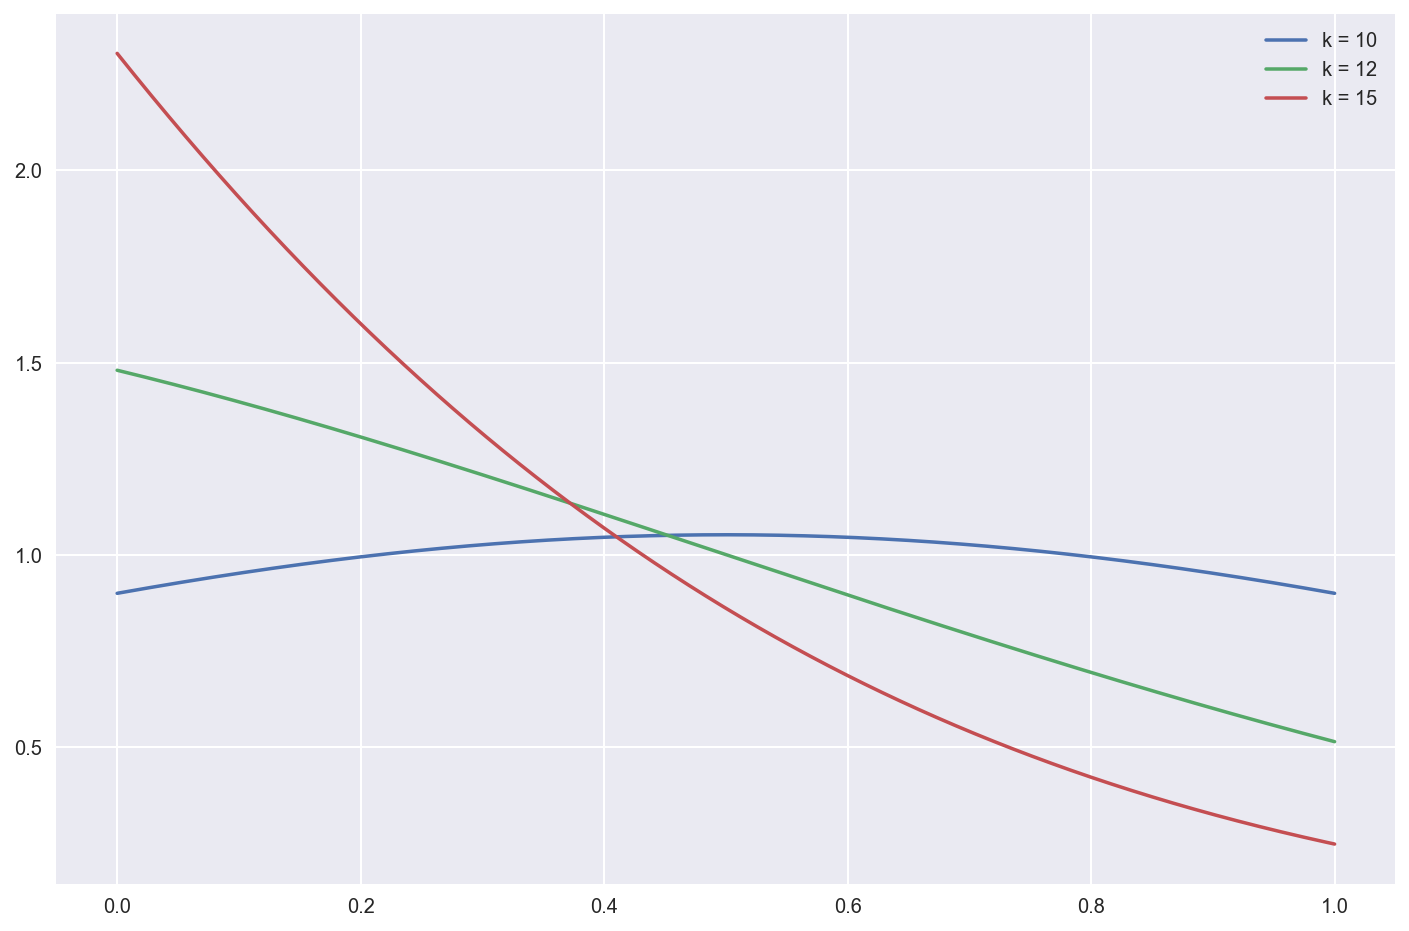
\includegraphics[width=0.8\textwidth]{img/distributions.png}
% \caption[Probability distribution of first sampled value]{Probability distribution of first sampled value $P(X_1 \mid \sum_{j=1}^{k} X_j = 5)$ for different values of $k$}
% \label{fig:dists}
% \end{figure}


% For the $t$-th value, we obtain an Irwin-Hall distribution on $k-t$ random variables with mean $v' - \sum_{j=1}^{t-1} x_j - \frac{k-t}{2}$.
% We have
% \[
%     P(X_t' = x_t' \mid \sum_{j=1}^{k} X_j' = v', X_1'=x_1', ...,X_{t-1}'=x_{t-1})'
% \]
% \[
%     = P(X_t' = x_t' \mid \sum_{j=t+1}^{k} X_j' = v' - \sum_{j=1}^{t} x_j', X_1'=x_1', ..., X_{t-1}'=x_{t-1}')
% \]
% \[
%     = \frac{P(\sum_{j=t+1}^{k} X_j' = v' - \sum_{j=1}^{t} x_j')}{P(\sum_{j=t}^{k} X_j' = v' - \sum_{j=1}^{t-1} x_j')}
% \]

% For $t = k$, $X_t$ converges to a single value, for $t = k-1$ it follows a uniform distribution and for $t = k-2$ a triangular distribution (as before all truncated and normalised).

% \todo[inline]{\url{https://stackoverflow.com/a/8068956} looks like a much easier approach to this problem}

% Naturally, if $\mathcal{A}$ has knowledge of the number of transactions $k$, they will learn some information from the observed amount(s) since the distribution $P(V \mid X)$ is a truncated Irwin-Hall distribution as discussed above.
% \todo{have some more work done on this but unsure whether to expand or remove altogether}

%coordinate along line
%sample from n-1-dimensional space
%if value $k$ is unknown to adversary, the distribution of possible values would be $P(V=v) = %\frac{\sum_{k=m}^{n} P(\sum_{i=1}^{k} X_i = v|X)}{n-m + 1}$, where $m=\left %\lceil{\frac{v-\sum_{x_i \in X} x_i}{\vmax}}\right \rceil + |X|$ and $n=\left %\lfloor{\frac{v-\sum_{x_i \in X} x_i}{\val_{min}}}\right \rfloor + |X|$, a sum of I-H %distributions across a larger set of possible values for \vtot.
%We do not try to analyse this distribution...
